\section{The Mean Value Theorem}\label{S:3.5.MeanValue}

\begin{goals}
\item In a setting where the average rate of change of a function $f$ is known for a given interval, is there a value where the function has an instantaneous rate of change equal to the average rate of change? 
\end{goals} 

%--------------------------------------
% SUBSECTION INTRODUCTION
%--------------------------------------
\subsection*{Introduction}

We motivate this section with the following question: Suppose you leave your house and drive to your friend's house in a city $120$ miles away, completing the trip in two hours.  At any point during the trip do you necessarily have to be going $60$ miles per hour?

In answering this question, it is clear that the \textit{average} speed for the entire trip is $60$ mph (i.e. $120$ miles in $2$ hours), but the question is whether or not your \textit{instantaneous} speed is ever exactly $60$ mph. More simply, does your speedometer ever read exactly $60$ mph?  The answer, under some very reasonable assumptions, is ``yes.''

Let's now see why this situation is in a calculus text by translating it into mathematical symbols.

First assume that the function $y = f(t)$ gives the distance (in miles) traveled from your home at time $t$ (in hours) where $0\le t\le 2$.  In particular, this gives $f(0)=0$ and $f(2)=120$.  The slope of the secant line connecting the starting and ending points $(0,f(0))$ and $(2,f(2))$ is therefore 
$$
\frac{\Delta f}{\Delta t} = \frac{f(2)-f(0)}{2-0} = \frac{120-0}{2} = 60 \, \text{mph}.
$$

The slope at any point on the graph itself is given by the derivative $\fp(t)$.  So, since the answer to the question above is ``yes,'' this means that at some time during the trip, the derivative takes on the value of $60$ mph.  Symbolically, 
$$
\fp(c) = \frac{f(2)-f(0)}{2-0} = 60
$$
for some time $0\le c \le 2.$ 

\begin{pa} \label{PA:3.5}
On a recent vacation trip, Michelle traveled 200 miles on a toll road in 3 hours. 
\ba
	\item Plot points on the graph to represent Michelle's distance traveled, d, at a given time, t, where $t=0$ represents the time she started driving on the toll road.  
	\item Draw a possible distance function, d(t), on the graph.  
	\item On the second graph, plot Michelle's velocity, v(t). What was her average velocity during the trip?
	\item Based on the distance function, does she ever exceed this average velocity? If yes, explain by finding a time where she exceeds the average velocity. If not, explain why.
	\item If Michelle had to stop to pay her toll when entering the toll road, does she ever exceed the average velocity?
\ea
\end{pa} 
\afterpa

\begin{marginfigure}[-1.75cm]
\subfloat{\margingraphics{figures/3_5_PA1a.pdf}} 

\subfloat{\margingraphics{figures/3_5_PA1b.pdf}}
\caption{Axes for plotting $y = d(t)$ and $y=v(t)=d'(t)$.} \label{fig:3.5.PA1}
\end{marginfigure} %PREVIEW needs written toll road problem?

%-----------------------------------------------
% SUBSECTION MEAN VALUE THEOREM
%-----------------------------------------------
\subsection*{The Mean Value Theorem}

Can we generalize the velocity problem above to any function? In other words, given any function $y=f(x)$ and a range $a\leq x \leq b$, does the value of the derivative at some point between $a$ and $b$ have to match the slope of the secant line connecting the points $(a,f(a))$ and $(b,f(b))$?  Or equivalently, does the equation 
$\fp(c) = \frac{f(b)-f(a)}{b-a}$ have to hold for some $a < c < b$?

The following Activity will explore what properties $f$ must possess in order for the equation 
$\fp(c) = \frac{f(b)-f(a)}{b-a}$ to hold for some $a < c < b$.

\begin{marginfigure}[2cm] % MARGIN FIGURE
\begin{center}
\subfloat[$f_1(x) = 1/x^2$]{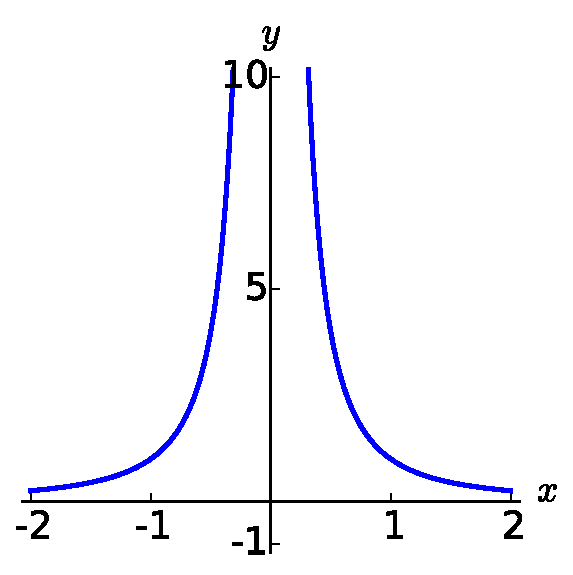
\includegraphics[scale=.3]{figs/3/activity351a.pdf}}
\hspace{.25cm}
\subfloat[$f_2(x) = |x|$]{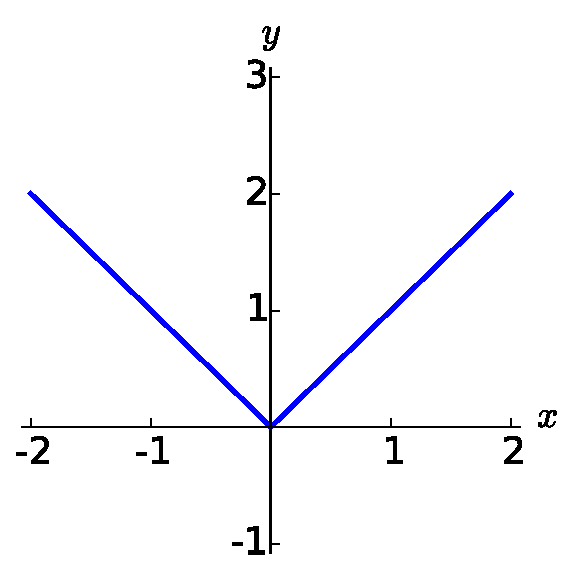
\includegraphics[scale=.3]{figs/3/activity351b.pdf}}
\caption{The functions $f_1(x) = 1/x^2$ and $f_2(x) = |x|$ used in Activity~\ref{A:3.5.1}}
\label{fig:act351}
\end{center}
\end{marginfigure}

\begin{activity} \label{A:3.5.1}  Consider functions 
$$f_1(x)=\frac{1}{x^2}\quad \text{and} \quad f_2(x) = |x|$$ 
with $a=-1$ and $b=1$ as shown in Figure~\ref{fig:act351}-(a) and -(b), respectively. 
\ba
 \item For $f_1(x)$, find the slope of the secant line connecting the points $(a,f(a))$ and $(b,f(b))$.
 \item Find a value $c$ in $(a,b)$ such that $f_1'(c)$ equals the slope of the secant line connecting the points $(a,f(a))$ and $(b,f(b))$. Was it possible to find $c$? If not, what went wrong?
  \item For $f_2(x)$, find the slope of the secant line connecting the points $(a,f(a))$ and $(b,f(b))$.
 \item Find a value $c$ in $(a,b)$ such that $f_2'(c)$ equals the slope of the secant line connecting the points $(a,f(a))$ and $(b,f(b))$. Was it possible to find $c$? If not, what went wrong?
	\ea
\end{activity}

\aftera % ACTIVITY

So what went ``wrong''?  It may not be surprising to find that the discontinuity of $f_1$ and the corner of $f_2$ play a role.  If our functions had been continuous and differentiable, would we have been able to find that special value $c$? This is our motivation for the following theorem.

\concept{The Mean Value Theorem of Differentiation\label{C:MVT}}  % CONCEPT
{Let $y=f(x)$ be a continuous function on the closed interval $[a,b]$ and differentiable on the open interval $(a,b)$. There exists a value $c$, $a < c < b$, such that \index{Mean Value Theorem!of differentiation}\index{derivative!Mean Value Theorem}
$$
\fp(c) = \frac{f(b)-f(a)}{b-a}.
$$
That is, there is a value $c$ in $(a,b)$ where the instantaneous rate of change of $f$ at $c$ is equal to the average rate of change of $f$ on $[a,b]$.} % end concept

Note that the reasons that the functions in Activity\ref{A:3.5.1} fail are indeed that $f_1$ has a discontinuity on the interval $[-1,1]$ and $f_2$ is not differentiable at the origin.

We will give a proof of the Mean Value Theorem below. To do so, we use another theorem, called Rolle's Theorem, stated here.

\concept{Rolle's Theorem\label{C:Rolles}} % CONCEPT
{Let $f$ be continuous on $[a,b]$ and differentiable on $(a,b)$, where $f(a) = f(b)$. There is some $c$ in $(a,b)$ such that $\fp(c) = 0.$\index{Rolle's Theorem}} % end CONCEPT

\begin{marginfigure}[1cm] % MARGIN FIGURE
\margingraphics{figures/figmvt3}
\caption{A graph of $f(x) = x^3-5x^2+3x+5$, where $f(a) = f(b)$. Note the existence of $c$, where $a<c<b$, where $\fp(c)=0$.}\label{fig:mvt3}
\end{marginfigure}

Consider Figure \ref{fig:mvt3} where the graph of a function $f$ is given, where $f(a) = f(b)$. It should make intuitive sense that if $f$ is differentiable (and hence, continuous) that there would be a value $c$ in $(a,b)$ where $\fp(c)=0$; that is, there would be a local maximum or minimum of $f$ in $(a,b)$. Rolle's Theorem guarantees at least one; there may be more. 

Rolle's Theorem is really just a special case of the Mean Value Theorem. If $f(a) = f(b)$, then the \textit{average} rate of change on $(a,b)$ is $0$, and the theorem guarantees some $c$ where $\fp(c)=0$. We will prove Rolle's Theorem, then use it to prove the Mean Value Theorem.\\

\proof (Rolle's Theorem) Let $f$ be differentiable on $(a,b)$ where $f(a)=f(b)$. We consider two cases. 

\noindent\textbf{Case 1:} Consider the case when $f$ is constant on $[a,b]$; that is, $f(x) = f(a) = f(b)$ for all $x$ in $[a,b]$. Then $\fp(x) = 0$ for all $x$ in $[a,b]$, showing there is at least one value $c$ in $(a,b)$ where $\fp(c)=0$.

\noindent\textbf{Case 2:} Now assume that $f$ is not constant on $[a,b]$. The Extreme Value Theorem guarantees that $f$ has a maximal and minimal value on $[a,b]$, found either at the endpoints or at a critical value in $(a,b)$. Since $f(a)=f(b)$ and $f$ is not constant, it is clear that the maximum and minimum cannot \textit{both} be found at the endpoints. Assume, without loss of generality, that the maximum of $f$ is not found at the endpoints. Therefore there is a $c$ in $(a,b)$ such that $f(c)$ is the maximum value of $f$. Thus $c$ must be a critical number of $f$; since $f$ is differentiable, we have that $\fp(c) = 0$, completing the proof of the theorem. \hfill $\square$\\

\proof (Mean Value Theorem) Define the function $$g(x) = f(x) - \frac{f(b)-f(a)}{b-a}x.$$  We know $g$ is differentiable on $(a,b)$ and  continuous on $[a,b]$ since $f$ is. We can show $g(a)=g(b)$ (it is actually easier to show $g(b)-g(a)=0$, which suffices). We can then apply Rolle's theorem to guarantee the existence of $c \in (a,b)$ such that $g'(c) = 0$.  But note that $$0= g'(c) = \fp(c) - \frac{f(b)-f(a)}{b-a} \ ;$$ hence $$\fp(c) = \frac{f(b)-f(a)}{b-a},$$ which is what we sought to prove.\hfill $\square$\\

Going back to the very beginning of the section, we see that the only assumption we would need about our distance function $f(t)$ is that it be continuous and differentiable for $t$ from $0$ to $2$ hours (both reasonable assumptions).  By the Mean Value Theorem, we are guaranteed a time during the trip where our instantaneous speed is $60$ mph. This fact is used in practice. Some law enforcement agencies monitor traffic speeds while in aircraft. They do not measure speed with radar, but rather by timing individual cars as they pass over lines painted on the highway whose distances apart are known. The officer is able to measure the \textit{average} speed of a car between the painted lines; if that average speed is greater than the posted speed limit, the officer is assured that the driver exceeded the speed limit at some time.

Note that the Mean Value Theorem is an \textit{existence} theorem. It states that a special value $c$ \textit{exists}, but it does not give any indication about how to find it.  To do so, we must be able to solve equations, which sometimes can be very difficult.  The following example demonstrates the process for finding a special value $c$.



\begin{example} \label{Ex:3.5.Eg1}
Consider $f(x) = x^3+5x+5$ on $[-3,3]$. Find $c$ in $[-3,3]$ that satisfies the Mean Value Theorem.

\solution
The average rate of change of $f$ on $[-3,3]$ is:
		$$\frac{f(3)-f(-3)}{3-(-3)} = \frac{84}{6} = 14.$$
		
We want to find $c$ such that $\fp(c) = 14$. We find $\fp(x) = 3x^2+5$. We set this equal to $14$ and solve for $x$. 
		\begin{align*}
		3x^2 +5 &= 14\\
		x^2  &= 3\\
		x &= \pm \sqrt{3} \approx \pm 1.732
		\end{align*}
		
We have found $2$ values $c$ in $[-3,3]$ where the instantaneous rate of change is equal to the average rate of change; the Mean Value Theorem guaranteed at least one. In Figure~\ref{F:3.5.Ex1} $f$ is graphed with a dashed line representing the average rate of change; the lines tangent to $f$ at $x=\pm \sqrt{3}$ are also given. Note how these lines are parallel (i.e., have the same slope) as the dashed line.

\end{example}

\begin{marginfigure}[-8cm]
\margingraphics{figures/figmvt4} %APEX ex83
\caption{Demonstrating the Mean Value Theorem in Example~\ref{Ex:3.5.Eg1}}\label{F:3.5.Ex1}
\end{marginfigure} % EXAMPLE

In the next activty, we examine two other results based on the Mean Value Theorem.


\begin{activity} \label{A:3.5.2}  In this activity, we will discuss two important consequences of the Mean Value Theorem.  
\ba
 \item Suppose $f'(x)=0$ for $x$ in $[a,b]$. What can we say about $f(x)$ on the interval $[a,b]$?
 \item Given two functions $f$ and $g$ defined on $[a,b]$ such that $f'(x)=g'(x)$ for all $x$ in $[a,b]$, what can we say about the functions themselves? How are $f$ and $g$ related?
	\ea
\end{activity}

\aftera % ACTIVITY

The Mean Value Theorem has practical use (for instance, the speed monitoring application mentioned before) in the sciences and other applications.  However, it turns out that when we need the Mean Value Theorem in mathematics, existence is all we need, and it is mostly used to advance other theory.

%--------------
% SUMMARY
%--------------
\begin{summary}
\item If $f$ is a continuous function on the closed interval $[a,b]$ and differentiable on the open interval $(a,b)$. There exists a value $c$, $a < c < b$, such that $\fp(c) = \frac{f(b)-f(a)}{b-a}$, i.e. the instantaneous rate of change of $f$ at $c$ is equal to the average rate of change of $f$ on $[a,b]$.
\end{summary}

%--------------
% EXERCISES
%--------------
\begin{adjustwidth*}{}{-2.25in}
\textbf{{\large Exercises}}
\setlength{\columnsep}{25pt}
\begin{multicols*}{2}
\noindent Terms and Concepts \small
\begin{enumerate}[1)]
\item Explain in your own words what the Mean Value Theorem states.
\item Explain in your own words what Rolle's Theorem states.
\end{enumerate} 

\noindent {\normalsize Problems} \small

\noindent{\bf In exercises 3--10, a function $f(x)$ and interval $[a,b]$ are given.  Check if Rolle's Theorem can be applied, and if so, find $c$ in $[a,b]$ such that $f'(c) = 0$.}

\begin{enumerate}[1),resume]
\item $f(x) = 6$ on $[-1,1]$.
\item $f(x) = 6x$ on $[-1,1]$.
\item $f(x) = x^2+x-6$ on $[-3,2]$.
\item $f(x) = x^2+x-2$ on $[-3,2]$.
\item $f(x) = x^2+x$ on $[-2,2]$.
\item $f(x) = \sin x$ on $[\pi/6,5\pi/6]$.
\item $f(x) = \cos x$ on $[0,\pi]$.
\item $\ds f(x) = \frac{1}{x^2-2x+1}$ on $[0,2]$.
\end{enumerate}

\noindent{\bf In exercises 11-20, a function $f(x)$ and interval $[a,b]$ are given Check if the Mean Value Theorem can be applied, and if so, find a value $c$ guaranteed by the Mean Value Theorem.}

\begin{enumerate}[1),resume]
\item $\ds f(x) = x^2+3x-1$ on $[-2,2]$.
\item $\ds f(x) = 5x^2-6x+8$ on $[0,5]$.
\item $\ds f(x) = \sqrt{9-x^2}$ on $[0,3]$.
\item $\ds f(x) = \sqrt{25-x}$ on $[0,9]$.
\item $\ds f(x) = \ln x$ on $[1,5]$.
\item $\ds f(x) = \tan x$ on $[-\pi/4,\pi/4]$.
\item $\ds f(x) = x^3-2x^2+x+1$ on $[-2,2]$.
\item $\ds f(x) = 2x^3-5x^2+6x+1$ on $[-5,2]$.
\item $\ds f(x) = \sin^{-1} x$ on $[-1,1]$.
\item $\ds f(x) =\frac{x^2-9}{x^2-1}$ on $[0,2]$.
\end{enumerate}

\begin{enumerate}[1),resume]
\item Show that the equation $6x^4 -7x+1 =0$ does not have more
than two distinct real roots.
%\begin{answer}
%Seeking a contradiction, suppose that we have 3 real roots, call them
%$a$, $b$, and $c$. By Rolle's Theorem, $24x^3-7$ must have a root on
%both $(a,b)$ and $(b,c)$, but this is impossible as $24x^3-7$ has only
%one real root.
%\end{answer}

\item Let $f(x)$ be differentiable on $\mathbb{R}$. Suppose that $f'(x) \ne
0$ for every $x$. Prove that $f$ has at most one real root.
%\begin{answer}
%Seeking a contradiction, suppose that we have 2 real roots, call them
%$a$, $b$. By Rolle's Theorem, $f'(x)$ must have a root on $(a,b)$, but
%this is impossible.
%\end{answer}


\item Two runners start a race at the same time and finish in a tie. Prove that at some time during the race they have the same speed.
\end{enumerate}

%------------------------------------------
% END OF EXERCISES ON FIRST PAGE
%------------------------------------------
\end{multicols*}
\end{adjustwidth*}

\afterexercises 

\cleardoublepage